\documentclass{article}


\usepackage[nottoc]{tocbibind}
\usepackage[backend=biber]{biblatex}
\bibliography{References.bib}


\usepackage{amsmath}
\usepackage{mathtools}
\usepackage{amsfonts}
\usepackage{amssymb}
\usepackage{standalone}
\usepackage{multirow}
\usepackage{graphicx}
\usepackage{caption}
\usepackage{bm}
\usepackage{gensymb}
\usepackage{siunitx}
\usepackage{float}
\usepackage{tikz}
\usepackage{tikz-3dplot}
\usetikzlibrary{calc}

\newcommand{\me}{\mathrm{e}}
\providecommand{\abs}[1]{\lvert#1\rvert} \providecommand{\norm}[1]{\lVert#1\rVert}



\title{Licenciate}
\author{Kajsa-My Blomdahl}
\date{October 2018}
\begin{document}

\maketitle

\tableofcontents

\section{Background}
\subsection{The Three-body Problem}
The $n$-body problem is a class of problems in physics which, in a highly general sense, consists of modelling the motion of $n$ objects, interacting through some physical force. In classical mechanics the equations of motion for $n$ point particles can be derived from Newton's second law of motion, which states that the rate of change in momentum for an object equals the force acting on it, or from analytical formulations such as Lagrangian and Hamiltonian mechanics, which consider scalar properties of motion like kinetic and potential energies. In the quantum regime, where the wave-like property of matter has to be taken into account, the state of an $n$-body system of is described by a total wave function, where the Hamiltonian operator generates the time evolution of the state as given by Schr{\"o}dinger's differential equation.

The core of the $n$-body problem is that the classical equations of motion and the Schr{\"o}dinger equation are not analytically solvable for more than two interacting particles. Consider the case where $n=3$. Albeit apparently simple, the configuration space for the three-body problem is six dimensional after separating out the center of mass motion. Three additional constants of motion can be provided by conservation of total angular momentum, which effectively reduces the problem to that of three coupled second order non-linear differential equations in the classical case and a three dimensional Schr{\"o}dinger equation for the quantum problem. The quest for a general solution to the classical three-body problem is renowned. As a recurrent muse to a number of great mathematicans during the past centuries, dating back to Newton himself, the three-body problem has been a catalysator for the development of analysis and the modern theory of dynamical systems \cite{Chenciner2015}. Although there are a number of special cases that have explicit solutions, nonlinear dynamical systems often display highly unpredictable behavoir due to sensitive dependence on initial conditions, i.e. they are chaotic. Different numerical approaches are used to solve this kind of problems nowadays but the computational load can be substantial. However, the quantum three-body problem is amenable to an analytic solution. 

Within the quantum realm of few-body systems the Faddeev and the Faddeev-Yakubovsky equations, which are equivalent formulations of the Schr{\"o}dinger equation for three- and four-body systems repectively, can be solved analytically by iteration for a few special cases \cite{Faddeev:1960su, Zubarev:1994}. For the three-body scattering problem, bound state solutions can exist in cases where all three two-body subsystems have short-ranged interactions, if at least two of these interactions are close to resonance. This is called the Efimov effect. 

\subsection{The Birth of Efimov Physics}
 In 1970, Vitaly Efimov predicted that resonant two-body forces could give rise to a series of bound energy levels in three-particle systems \cite{Efimov:1970zz}. When the short-ranged two-body forces approached resonance, he found a universal long-range three-body attraction emerging, giving rise to an infinite number of trimer states with binding energies obeying a discrete scaling law at resonance.  
 
 Efimov proposed that attractive three-body interaction appearing in systems with resonant short-ranged interactions and repulsive Coulomb forces could explain the binding of three particle nuclei such as the three nucleon triton $\prescript{3}{}{\mathrm{H}}$ and the triple-alpha Hoyl state of $\prescript{12}{}{\mathrm{C}}$.

The notion of Efimov physics comprise a range of universal phenomena that occurs in few-body systems exibiting the Efimov effect. Short-ranged forces are commonly occuring in nature and few-body effects are expected to appear in a broad range of physical sytems. Developments in the theory of few-body quantum systems is important since it would bridge existing well developed models of treating one- and two-body sytems with the statistical methods used to describe many-body systems, and it may give insight... 

\section{Introduction} 
\subsection{Three-body Theory}
A short reveiw concerning some important aspects of quantum mechanical systems and two-body scattering will follow in order to set the stage for a discussion of quantum effects in few-body systems in general and Efimov states in three-body systems in particular. 

\paragraph{Entering the quantum regime}
All particles of matter exhibit wave-like properties. The wave length of a particle with momentum $p$ is given by the de Broglie equation

\begin{equation} \label{eq:1}
\lambda = \frac{h}{p} = \frac{h}{mv}
\end{equation}
where $h$ is the Planck constant. The wave characteristics of matter grows with increasing de Broglie wavelength. When the wavelength is sufficently large, classical physics no longer applies and the system has reached the quantum regime. From \eqref{eq:1} it is evident that this is true for particles that are either very small or very slow. In an ultracold quantum gas, the atoms are cooled down to a point where they move so slowly that the increased uncertainty in position for the individual atoms eventually becomes so large that they start to overlap and the atoms cannot be viewed as individual particles but as a correlated wave. In this ultracold regime, when the de Broglie wavelength is larger than the average space between the atoms their behaviour are governed by quantum mechanics. 
 
\subsubsection{Two-body Interactions}
Atomic interactions are short ranged and in the ultracold regime their de Broglie wavelength is larger than the typical range of interaction. Consequentely, their interactions can no longer be described as pointlike collisions. Instead, scattering process in this regime is governed by the scattering length, which intuitively can be described as the length for which a hard sphere of the same radius would scatter off. The scattering length $a$ is defined as

\begin{equation} \label{eq:2}
\lim_{k \to 0} k \cot \delta(k) = -\frac{1}{a}
\end{equation}
where $k$ is the wave number and $\delta(k)$ is the phase shift.

\subsubsection{The Three-body Problem}
The three-body scattering problem can be solved by the three-body Schr{\"o}dinger equation or by the Faddeev equation. Solving the Faddeev equation is equivalent to solving the Schr{\"o}dinger equation 
There are two main approaches for the three-body scattering problem. Either by solving the three-body Schr{\"o}dinger equation means of the Faddeev equation, which is equivalent to solving the three-body Schr{\"o}dinger equation in configuration space   
There are two general approaches for solving the three-body Schr{\"o}dinger equation, either by treating the particles collectively as a whole, or to treat them idependently. The hyperspherical collective coordinate method. The adiabatic hyperspherical method.

\subsection{Experimental Evidence}
\subsubsection{Efimov Trimers in Atomic Systems}
Ultracold atomic clouds provided the first staging ground for exploring Efimov physics and related few-body phenomena because of the ability to control atom-atom interactions by an external field. In these extremely dilute gases, with densities $n$, the probability for collisions can reach unity by tuning the s-wave scattering length to the unitary regime $n\abs{a^3}\gg1$. In experiments with trapped ultracold atomic and molecular gases of alkali atoms with tunable two-body interactions, the existance of Efimov trimers have been inferred from resonantly enhanced loss rates, either in atomic three-body recombination processes at negative $a$, when the Efimov state couples to the triatomic threshold, or in atom-dimer relaxation processes. 
\paragraph{Alkali atomic gases} 
The first observations of an Efimov state was in an ultracold gas of $\prescript{133}{}{\mathrm{Cs}}$ was reported in 2006 by the group of Grimm and coworkers \cite{Grimm:2006}. Later experiments have strengthen the evidence of these elusive states and in 2014 observations of the first exited Efimov state confirmed the theoretically predicted universal scaling properties of two succesive Efimov states \cite{Huang2014}. Efimov resonances in homogenic gases with other atomic species have been observed including $\prescript{85}{}{\mathrm{Rb}}$, $\prescript{39}{}{\mathrm{K}}$, $\prescript{7}{}{\mathrm{Li}}$, and three component fermi gases of $\prescript{6}{}{\mathrm{Li}}$. Also mixtures mixtures of $\prescript{41}{}{\mathrm{K}}$ and $\prescript{87}{}{\mathrm{Rb}}$ has been investigated.

\paragraph{Helium trimers}
Helium is a prime candidate to study Efimov physics with a more direct approach. The ground state of the helium trimer is not an Efimov state. However the first and second exited trimer have Efimov characteristics. Coulomb explosion imaging of helium trimers have revealed the geometric form of the trimers. \cite{Kunitski:2015qth}

\subsubsection{Efimov States in Nuclei }

\subsubsection{Four-body Recombination connected to Efimov Trimers} 
The Efimov scenario is even richer. In connection to an Efimov trimer, a pair of four-body states can form when a fourth atom approach. In accordance with the theoretical predictions, strong evidence for the existance of a pair of four-body states was provided in 2009 \cite{Grimm:2009}. 

\section{Theoretical Methods} 
Two-body scattering processes concern two differnt situations, elastic and inelastic collisions. For the three-body problem, solving the three-body Schr{\"o}dinger equation is more involved. The enhanced complexity is mainly due to the increased number of fragmentation channels in the scattering processes. In addition to the triatomic fragmentation channel (1+1+1), there are three possible atom-dimer fragmenation channels (1+2). There are different routes of solving the three-body problem. However, most approaches start with the same steps. This includes separating out the  center of mass motion and then defining a set of relative  coordinates. A convenient choice for the three-body problem is mass normalized Jacobi coordinates, since it removes the mass factors in the kinetic energy operator.     

\begin{figure}
	\centering
	 \documentclass{standalone}
 \usepackage{tikz}
 \usepackage{tikz-3dplot}
 \usetikzlibrary{calc}
 
 \begin{document}
 
  %Angle Definitions
%-----------------

%set the plot display orientation
%synatax: \tdplotsetdisplay{\theta_d}{\phi_d}
\tdplotsetmaincoords{60}{110}

%define polar coordinates for some vector
%TODO: look into using 3d spherical coordinate system
\pgfmathsetmacro{\rvec}{.8}
\pgfmathsetmacro{\thetavec}{30}
\pgfmathsetmacro{\phivec}{80}

\pgfmathsetmacro{\rveca}{.8}
\pgfmathsetmacro{\thetaveca}{50}
\pgfmathsetmacro{\phiveca}{320}

\pgfmathsetmacro{\rvecb}{.8}
\pgfmathsetmacro{\thetavecb}{50}
\pgfmathsetmacro{\phivecb}{40}


%start tikz picture, and use the tdplot_main_coords style to implement the display 
%coordinate transformation provided by 3dplot
\begin{tikzpicture}[scale=5,tdplot_main_coords]

%set up some coordinates 
%-----------------------
\coordinate (O) at (0,0,0);

%determine a coordinate (P) using (r,\theta,\phi) coordinates.  This command
%also determines (Pxy), (Pxz), and (Pyz): the xy-, xz-, and yz-projections
%of the point (P).
%syntax: \tdplotsetcoord{Coordinate name without parentheses}{r}{\theta}{\phi}
\tdplotsetcoord{P}{\rvec}{\thetavec}{\phivec}
\tdplotsetcoord{F}{\rveca}{\thetaveca}{\phiveca}
\tdplotsetcoord{R}{\rvecb}{\thetavecb}{\phivecb}
\coordinate (M) at ($ (P) !.5! (R) $);


%draw figure contents
%--------------------

%draw the main coordinate system axes
\draw[thick,->] (0,0,0) -- (1,0,0) node[anchor=north east]{$x$};
\draw[thick,->] (0,0,0) -- (0,1,0) node[anchor=north west]{$y$};
\draw[thick,->] (0,0,0) -- (0,0,1) node[anchor=south]{$z$};
%draw a vector from origin to point (P) 
\draw[-stealth,color=red] (O) -- (P) node[pos=0.5, right]{$x_{i}$};
\draw[-stealth,color=red] (O) -- (F) node[pos=0.5, right]{$x_{k}$};
\draw[-stealth,color=red] (O) -- (R) node[pos=0.5, right]{$x_{j}$};

\draw[thick,->,color=blue] (P) -- (R) node[pos=0.5, right]{$x_{ij}$};
\draw[thick,->,color=blue] (M) -- (F) node[pos=0.5, below]{$x_{ij,k}$};
%\draw[-stealth,color=red] (O) -- (R);

%draw projection on xy plane, and a connecting line
\draw[dashed, color=red] (O) -- (Pxy);
\draw[dashed, color=red] (P) -- (Pxy);

\draw[dashed, color=red] (O) -- (Fxy);
\draw[dashed, color=red] (F) -- (Fxy);

\draw[dashed, color=red] (O) -- (Rxy);
\draw[dashed, color=red] (R) -- (Rxy);

%draw the angle \phi, and label it
%syntax: \tdplotdrawarc[coordinate frame, draw options]{center point}{r}{angle}{label options}{label}
\tdplotdrawarc{(O)}{0.8}{0}{\phivec}{anchor=north}{$\phi_i$}
\tdplotdrawarc{(O)}{0.2}{0}{\phiveca}{anchor=north}{$\phi_j$}
\tdplotdrawarc{(O)}{0.4}{0}{\phivecb}{anchor=north}{$\phi_k$}


%set the rotated coordinate system so the x'-y' plane lies within the
%"theta plane" of the main coordinate system
%syntax: \tdplotsetthetaplanecoords{\phi}
\tdplotsetthetaplanecoords{\phivec}

%draw theta arc and label, using rotated coordinate system
\tdplotdrawarc[tdplot_rotated_coords]{(0,0,0)}{0.8}{0}{\thetavec}{anchor=south west}{$\theta_i$}

%draw some dashed arcs, demonstrating direct arc drawing
\draw[dashed,tdplot_rotated_coords] (\rvec,0,0) arc (0:90:\rvec);
\draw[dashed] (\rvec,0,0) arc (0:90:\rvec);


\tdplotsetthetaplanecoords{\phiveca}
\tdplotdrawarc[tdplot_rotated_coords]{(0,0,0)}{0.8}{0}{\thetaveca}{anchor=south east}{$\theta_k$}


%draw some dashed arcs, demonstrating direct arc drawing
\draw[dashed,tdplot_rotated_coords] (\rveca,0,0) arc (0:90:\rveca);
\draw[dashed] (\rveca,0,0) arc (0:\phiveca:\rveca);

\tdplotsetthetaplanecoords{\phivecb}
\tdplotdrawarc[tdplot_rotated_coords]{(0,0,0)}{0.8}{0}{\thetavecb}{anchor=south east}{$\theta_j$}


%draw some dashed arcs, demonstrating direct arc drawing
\draw[dashed,tdplot_rotated_coords] (\rvecb,0,0) arc (0:90:\rvecb);
\draw[dashed] (\rvecb,0,0) arc (0:90:\rvecb);


\end{tikzpicture}
\end{document}
	\caption{Spatial positions of three particles.}
	\label{fig:1}
\end{figure}

\subsection{Mass Normalized Jacobi Coordinates}
The spatial position of three particles in $\mathbb{R}^3$ are fixed by nine coordinates $x_{\alpha}^{i}$, where $i(=1,2,3)$ labels the particles, and $\alpha(=1,2,3)$ their Cartesian space coordinates, respectively. Let $\mathbf{x}_i$ and $m_{i}$ be the position vector and mass of the $i$th particle in the laboratory frame. If the total mass $M$, the three particle reduced mass $\mu_{3}$, and the normalizing constants $d_{k}$ $(k=1,2,3)$ are given by 

\begin{align}
M &= \sum_{i=1}^{3}m_i,  \label{eq:3,1} \\
\mu^2 &= \prod_{i=1}^{3}m_i/M,  \label{eq:3,2}\\
d_k^2 &= \frac{m_k}{\mu}\frac{(m_i+m_j)}{M}.  \label{eq:3,3}
\end{align}
Then a set of mass scaled Jacobi coordinates and the center of mass coordinate can be defined as

\begin{align}
\mathbf{r}_k &= d^{-1}_k(\mathbf{x}_{j}-\mathbf{x}_{i}),  \label{eq:4,1} \\
\mathbf{R}_k &= d_k\Big[\mathbf{x}_{k}-\frac{(m_{i}\mathbf{x}_{i}+m_{j}\mathbf{x}_{j})}{m_{i}+m_{j}}\Big],  \label{eq:4,2}\\
\mathbf{X}_{cm} &= \frac{1}{M} \sum_{i=1}^{3} m_{i} \mathbf{x}_{i},  \label{eq:4,3}
\end{align}   
where, the indices $i,j,k$ are cyclic permutations of $(1,2,3)$. Subsequently, the kinetic energy operator for the three particles in the laboratory frame, as given by 

\begin{equation}\label{eq:5}
\hat{T} = -\frac{\hbar^2}{2} \sum_{i=1}^{3} m_{i}^{-1} \nabla^{2}_{\mathbf{x}_{i}}, 
\end{equation}
will transform into

\begin{equation}\label{eq:6}
\hat{T} = -\frac{\hbar^2}{2\mu} \Big(\nabla^{2}_{\mathbf{r}_{k}}+\nabla^{2}_{\mathbf{R}_{k}}\Big) - \frac{\hbar^2}{2 M}\nabla^{2}_{\mathbf{X}_{cm}}. 
\end{equation}
The center of mass motion decouples from the internal equations of motion and thus will not be considered further. There are three possible ways to construct the Jacobi coordinates described above, see Figure \ref{fig:2}. Each set transforms into one of the other by exchange of particles. In cases with non-mass-scaled coordinates we define the particle permutations operators as 

\begin{figure}
	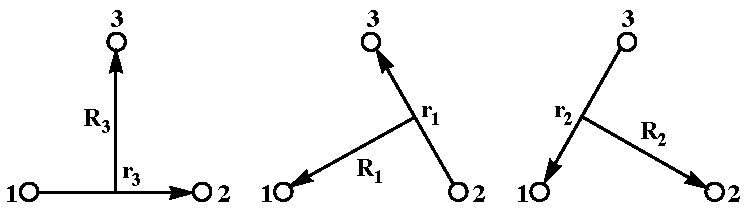
\includegraphics[width=\linewidth]{jacobii.pdf}
	\caption{Three different Jacobi coordinates.}
	\label{fig:2}
\end{figure}

\begin{equation}
\hat{P}_{13} = \left \{ \begin{aligned}
\mathbf{r} \, ' &= \mathbf{x}_2 - \mathbf{x}_3 &&= \frac{1}{2}\mathbf{r} - \mathbf{R} \\
\mathbf{R} \, ' &= \mathbf{x}_1 - \frac{1}{2}(\mathbf{x}_3 + \mathbf{x}_2) &&= -\frac{1}{2}(\frac{3}{2} \mathbf{r} + \mathbf{R}) 
\end{aligned}
\right.
\end{equation}

\begin{equation}
\hat{P}_{23} = \left \{ \begin{aligned}
\mathbf{r} \, '' &= \mathbf{x}_3 - \mathbf{x}_1 &&= \frac{1}{2}\mathbf{r} + \mathbf{R} \\
\mathbf{R} \, '' &= \mathbf{x}_2 - \frac{1}{2}(\mathbf{x}_1 + \mathbf{x}_3) &&= -\frac{1}{2} (\frac{3}{2} \mathbf{r} - \mathbf{R})
\end{aligned}
\right.
\end{equation}
For describing permutations in a system with mass-scaled coordinates it is useful to introduce angles defined by the particle masses \cite{Smith1962}\cite{Johnson1980}. If an even permutation $(ijk)$ of the set $(123)$ is considered, then the obtuse angle $\beta_{ij}$ has the properties

\begin{subequations}
	\begin{align}
	&\beta_{ij} = -\beta_{ji}, \quad \beta_{ii} = 0,\\
	&\tan\beta_{ij} = -m_k/\mu,\\
	&d_{i}d_{j} \sin\beta_{ij} = 1,\\
	&d_{i}d_{j} m_{k} \cos\beta_{ij} = -\mu,\\
	&\beta_{12}+\beta_{23}+\beta_{31} = 2\pi
	\end{align}
\end{subequations}
Orthogonal transformations within the coordinate set are then given by 

\begin{equation}
\begin{pmatrix}
\mathbf{r}_j\\
\mathbf{R}_j
\end{pmatrix}
=
\begin{pmatrix}
\cos\beta_{ij} & \sin\beta_{ij}\\
-\sin\beta_{ij} & \cos\beta_{ij}
\end{pmatrix}
\begin{pmatrix}
\mathbf{r}_i\\
\mathbf{R}_i
\end{pmatrix}
\end{equation}   
From hereon we choose one set to work in and suppress all vector indices.

\subsection{The Hyperspherical Method}
The next common step in the theoretical framework to describe systems of three particles is to introduce hyperspherical coordinates. The components of the two vectors $\mathbf{r}$ and $\mathbf{R}$ are combined into a single, six-dimensional position vector $\mathbf{q}$. The components of this vector can be regarded as the cartesian components of a point in $\mathbb{R}^{6}$. The motion of the three particle system is thus equivalent to the motion of a single particle, with the reduced mass $\mu$, in six-dimensional Euclidean space. The polar coordinates of this point particle are given by one hyperradial coordinate, $\rho$, and five hyperangular coordinates, collectively labelled $\Omega$. Three of these hyperangles are the Euler angles associated with the orientation of the body fixed frame (i.e., the triangle formed by the three particles) in three-dimensional space, these are called external coordinates. The remaing two hyperangles describe the shape of the triangle, and the hyperradius describes the overall size of the system, these coordinates are the internal coordinates of the system. For the three-body problem, the hyperradius is defined by

\begin{equation}
\rho = \Big(\mathbf{r}^{2} + \mathbf{R}^{2}\Big)^{1/2}, \quad 0\leq \rho < \infty.
\end{equation} 
Hyperspherical coordinates are useful for describing fragmentation problems. Fragmentations processes of the system into any one of the possible channels are described by the hyperradius becoming very large $(\rho \rightarrow \infty)$, while the hyperangles distinguishes between the different fragmentation channels. The hyperradius invariant under both rotations and particle permutation. However, there are various ways to define the hyperangles and they are not in general invariant under particle permutations. The most common choises of parametrizing this hypersphere fall into two distinct categories: Delves coordinates, and (democratic) Smith-Whitten coordinates. 

\subsubsection{Delves Coordinates}
Delves coordinates where originally developed to treat nuclear three-body problems. Delves coordinates are adapted to collinear atom-diatom collisions and they are regular polar coordinates, where

\begin{subequations}
	\begin{align}
		r_{k} &= \rho \sin(\alpha_{k})\\
		R_{k} &= \rho \cos(\alpha_{k}).
	\end{align}
\end{subequations}
The Delves hyperangle $\alpha_{k}$ is then defined by

\begin{equation}
	\alpha_{k} = \arctan\bigg(\frac{r_{k}}{R_{k}}\bigg), \quad 0\leq \alpha_{k} < \frac{\pi}{2}.
\end{equation}
This coordinate set corresponds to the reactant arrangement when particle $k$ scatters of the weakly bound particles $i-j$. These
Numerical difficulties arise with Delves hyper angles when permutation symmetries for three identical particles is considered.

\subsubsection{Smith-Whitten Coordinates}
Principel axis methods are characterized by the use of a single hyperspherical coordinate system that treats all three arragements of particles equivalently. 


\begin{subequations}
Introducing hyperspherical coordinates:
\begin{align}
        x &= \sqrt{2} \rho \sin(\alpha)\\
        y &= \sqrt{\frac{3}{2}} \rho \cos(\alpha)\\
\end{align}
\end{subequations}

Hyperspherical coordinates:
\[\arraycolsep=1.4pt\def\arraystretch{2.2}
     \left. \begin{array}{lr}
        \rho = \displaystyle \Big( \frac{1}{2}x^2 + \frac{2}{3}y^2 \Big) ^{1/2} &,  0\leq \rho < \infty\\
        \tan{\alpha} = \displaystyle \frac{\sqrt{3}}{2} \frac{x}{y} &,  0\leq \alpha < \frac{\pi}{2}\\
        \cos{\theta} = \displaystyle \frac{\vec{x} \cdot \vec{y}}{xy} &,  0\leq \theta < \pi
        \end{array}\right.
  \]

\begin{subequations}
Jacobi vectors:
\begin{align}
        x' &= \Big(\frac{1}{4} x^2 +y^2 -\vec{x} \cdot \vec{y}\Big)^{1/2} = \frac{\rho}{\sqrt{2}} \big( \sin^2(\alpha) + 3\cos^2(\alpha) - \sqrt{3}\sin(2\alpha)\cos{\theta}\big)^{1/2}\\
        x'' &= \Big(\frac{1}{4} x^2 +y^2 +\vec{x} \cdot \vec{y}\Big)^{1/2} = \frac{\rho}{\sqrt{2}} \big( \sin^2(\alpha) + 3\cos^2(\alpha) + \sqrt{3}\sin(2\alpha)\cos{\theta}\big)^{1/2}
\end{align}
\end{subequations}

Volume element from the transformation is $dr_1dr_2dr_3=3/2dxdydX_{cm}$.\\


(The massweighted Schr{\"o}dinger equation of a N-body system with position vectors $\mathbf{r}_k$ and masses $m_k$, ($k=1,...,N$), is given by)

\begin{equation}
\Bigg(-\frac{\hbar^2}{2} \sum_{k=1}^{N} m^{-1}_{k} \nabla^{2}_{\mathbf{r}_{k}} \Psi + V\Psi = E \Psi \Bigg)
\end{equation}

where the Laplacian is

\begin{equation}
\nabla^{2} = \Big( \frac{1}{r^2}\partial_{r} \big(r^2 \partial_{r}\big) - \frac{1}{\sin(\theta)} \partial_{\theta} \big( \sin(\theta) \partial_{\theta} \big) + \frac{1}{\sin^2{\theta}} \partial^{2}_{\phi} \Big) = \Big( \frac{1}{r^2} \partial_{r} \big( r^2 \partial_{r} \big) + \frac{L^2}{\hbar^2} \Big)
\end{equation}

The kinetic energy for three particles with identical masses is given by

\begin{equation}
\hat{T} = -\frac{\hbar^2}{2m}( \nabla^{2}_{r_1} + \nabla^{2}_{r_2} + \nabla^{2}_{r_3} )
\end{equation}

in hyperspherical coordinates this becomes 

\begin{equation}
\hat{T} = -\frac{\hbar^2}{2m}( 2\nabla^{2}_{x} + \frac{3}{2}\nabla^{2}_{y} + \frac{1}{3}\nabla^{2}_{X_{cm}} ),
\end{equation}

where

\begin{subequations}
\begin{align}
	\nabla^2_{x} &= \frac{1}{x^2}\frac{\partial}{\partial x} \Big( x^2 \frac{\partial}{\partial x} \Big) - \frac{\hat{l}^2_{x}}{x^2} = \frac{2}{x}\frac{\partial}{\partial x} + \frac{\partial^2}{\partial x^{2}} - \frac{\hat{l}^{2}_{x}}{x^2}\\
	\nabla^2_{y} &= \frac{1}{y^2}\frac{\partial}{\partial y} \Big( y^2 \frac{\partial}{\partial y} \Big) - \frac{\hat{l}^2_{y}}{y^2} = \frac{2}{y}\frac{\partial}{\partial y} + \frac{\partial^2}{\partial y^{2}} - \frac{\hat{l}^{2}_{y}}{y^2}
\end{align}
\end{subequations}

If spin interactions are excluded the total orbital angular momentum is zero and we have 

\begin{subequations}
\begin{align}
\hat{l}^{2}_{x} = \hat{l}^{2}_{y} = -\frac{1}{\sin(\theta)} \frac{\partial}{\partial{\theta}} \Big( \sin(\theta) \frac{\partial}{\partial{\theta}} \Big)
\end{align}
\end{subequations}



\begin{subequations}
\begin{align*}
        \frac{\partial \alpha}{\partial x} &= \frac{1}{\sqrt{2} \rho} \cos(\alpha), \quad \frac{\partial \rho}{\partial x} = \frac{1}{\sqrt{2}} \sin(\alpha) \\
        \frac{\partial \alpha}{\partial y} &= -\frac{\sqrt{6}}{3 \rho} \sin(\alpha), \quad \frac{\partial \rho}{\partial y} = \sqrt{\frac{2}{3}} \cos(\alpha)
\end{align*}
\end{subequations}

\begin{subequations}
\begin{align*}
        \frac{\partial}{\partial x}        &= \frac{\partial\alpha}{\partial x} \frac{\partial}{\partial\alpha} +  \frac{\partial\rho}{\partial x} \frac{\partial}{\partial\rho} \\
        \frac{\partial^2}{\partial x^2} &= \frac{1}{2} \Big( \frac{1}{\rho} \cos(\alpha) \frac{\partial}{\partial\alpha} + \sin(\alpha) \frac{\partial}{\partial\rho}\Big) \Big( \frac{1}{\rho} \cos(\alpha) \frac{\partial}{\partial\alpha} + \sin(\alpha) \frac{\partial}{\partial\rho}\Big) \\
                                                     &= \frac{1}{2} \Big[ \frac{1}{\rho^2} \cos(\alpha) \frac{\partial}{\partial\alpha} \Big( \cos(\alpha) \frac{\partial}{\partial\alpha} \Big) + \frac{1}{\rho} \cos(\alpha) \frac{\partial}{\partial\alpha} \Big( \sin(\alpha) \frac{\partial}{\partial\rho} \Big) + \sin(\alpha) \frac{\partial}{\partial\rho} \Big( \frac{1}{\rho} \cos(\alpha) \frac{\partial}{\partial\alpha} + \sin(\alpha) \frac{\partial}{\partial\rho} \Big)   \Big] \\
                                                     &= \frac{1}{2} \Big[ -\frac{2}{\rho^2} \cos(\alpha) \sin(\alpha) \frac{\partial}{\partial\alpha} + \frac{1}{\rho^2} \cos^2(\alpha) \frac{\partial^2}{\partial\alpha^{2}} + \frac{1}{\rho} \cos^2(\alpha) \frac{\partial}{\partial\rho} + \frac{2}{\rho} \cos(\alpha)\sin(\alpha) \frac{\partial^2}{\partial\alpha \partial\rho} + \sin^2(\alpha) \frac{\partial^2}{\partial\rho^{2}}\Big] \\
                                                     &= \frac{1}{2} \Big[ \frac{1}{\rho^2} \cos^2(\alpha) \frac{\partial^2}{\partial\alpha^{2}} - \frac{1}{\rho^2} \sin(2\alpha) \frac{\partial}{\partial\alpha} + \sin^2(\alpha) \frac{\partial^2}{\partial\rho^{2}} + \frac{1}{\rho} \cos^2(\alpha) \frac{\partial}{\partial\rho} + \frac{1}{\rho} \sin(2\alpha) \frac{\partial^2}{\partial\alpha \partial\rho}\Big]
\end{align*}
\end{subequations}

\begin{subequations}
\begin{align*}
        \frac{\partial}{\partial y}        &= \frac{\partial\alpha}{\partial y} \frac{\partial}{\partial\alpha} +  \frac{\partial\rho}{\partial y} \frac{\partial}{\partial\rho} \\
        \frac{\partial^2}{\partial y^2}&= \Big( -\frac{\sqrt{6}}{3\rho} \sin(\alpha) \frac{\partial}{\partial\alpha} + \sqrt{\frac{2}{3}} \cos(\alpha) \frac{\partial}{\partial\rho}\Big)  \Big( -\frac{\sqrt{6}}{3}  \sin(\alpha) \frac{\partial}{\partial\alpha} + \sqrt{\frac{2}{3}} \cos(\alpha) \frac{\partial}{\partial\rho}\Big) \\
                                                    &= \frac{2}{3} \Big[ \frac{1}{\rho^2} \sin(\alpha) \frac{\partial}{\partial\alpha} \Big( \sin(\alpha) \frac{\partial}{\partial\alpha}\Big) - \frac{1}{\rho} \sin(\alpha) \frac{\partial}{\partial\alpha} \Big( \cos(\alpha) \frac{\partial}{\partial\rho} \Big) - \cos(\alpha) \frac{\partial}{\partial\rho} \Big( \frac{1}{\rho} \sin(\alpha) \frac{\partial}{\partial\alpha} \Big) + \cos^2(\alpha)\frac{\partial^2}{\partial\rho^{2}} \Big] \\
                                                    &= \frac{2}{3} \Big[ \frac{2}{\rho^2} \sin(\alpha) \cos(\alpha) \frac{\partial}{\partial\alpha} + \frac{1}{\rho^2} \sin^2(\alpha)\frac{\partial^2}{\partial\alpha^{2}} + \frac{1}{\rho} \sin^2(\alpha) \frac{\partial}{\partial\rho} - \frac{2}{\rho}\sin(\alpha)\cos(\alpha) \frac{\partial^2}{\partial\alpha \partial\rho} +\cos^2(\alpha)\frac{\partial^2}{\partial\rho^{2}}  \Big]\\
                                                    &= \frac{2}{3} \Big[ \frac{1}{\rho^2} \sin^2(\alpha)\frac{\partial^2}{\partial\alpha^{2}} + \frac{1}{\rho^2} \sin(2\alpha)\frac{\partial}{\partial\alpha} + \cos^2(\alpha) \frac{\partial^2}{\rho^2} - \frac{1}{\rho} \sin(2\alpha) \frac{\partial^2}{\partial\alpha \partial\rho} \Big]
\end{align*}
\end{subequations}

\begin{subequations}
\begin{align*}
	2\nabla^{2}_{x} + \frac{3}{2}\nabla^{2}_{y} &= \frac{4}{x}\frac{\partial}{\partial x} +  \frac{3}{y} \frac{\partial}{\partial y}  +2\frac{\partial^2}{\partial x^{2}} + \frac{3}{2} \frac{\partial^2}{\partial y^{2}} - 2\frac{\hat{l}^{2}_{x}}{x^2} - \frac{3}{2}\frac{\hat{l}^{2}_{y}}{y^2}\\
									&= \frac{4}{\rho^2} \cot(2\alpha) \frac{\partial}{\partial\alpha} + \frac{5}{\rho} \frac{\partial}{\partial\rho} + \frac{1}{\rho^2} \frac{\partial^2}{\partial\alpha^2} + \frac{\partial^2}{\partial\rho^2} + \frac{4}{\rho^2 \sin^2(2\alpha)\sin(\theta)} \frac{\partial}{\partial\theta} \Big( \sin(\theta) \frac{\partial}{\partial{\theta}} \Big)\\
									&= \frac{1}{\rho^5}\frac{\partial}{\partial\rho} \Big( \rho^5 \frac{\partial}{\partial\rho} \Big) + \frac{1}{\rho^2 \sin^2(2\alpha)}  \Big( \frac{\partial}{\partial\alpha} \sin^2(2\alpha) \frac{\partial}{\partial\alpha} + \frac{4}{\sin(\theta)} \frac{\partial}{\partial\theta} \Big)
\end{align*}
\end{subequations}

The kinetic energy operators expressed in Delves hypersherical coordinates is thus

\begin{equation}
\hat{T} = \hat{T}_{\rho} +  \hat{T}_{\alpha}+\hat{T}_{\theta} 
\end{equation}

where

\begin{subequations}
\begin{align*}
\hat{T}_{\rho} &= -\frac{\hbar^2}{2m} \Big[ \frac{1}{\rho^5}\frac{\partial}{\partial\rho} \Big( \rho^5 \frac{\partial}{\partial\rho} \Big)  \Big]\\ 
                      &= -\frac{\hbar^2}{2m} \Big[ \rho^{-5/2} \Big( \rho^{5/2} \frac{5}{\rho} \frac{\partial}{\partial\rho} + \rho^{5/2} \frac{\partial^2}{\partial\rho^2} \Big) \rho^{-5/2} \rho^{5/2} \Big]\\
                      &= -\frac{\hbar^2}{2m} \rho^{-5/2} \Big[  -\frac{15}{4} \frac{1}{\rho^2} + \frac{\partial^2}{\partial\rho^2} \Big] \rho^{5/2}\\ \\
\hat{T}_{\alpha} &= -\frac{\hbar^2}{2m}  \frac{1}{\rho^2 \sin^2(2\alpha)}  \Big[ \frac{\partial}{\partial\alpha} \sin^2(2\alpha) \frac{\partial}{\partial\alpha} \Big]\\ 
                      &= -\frac{\hbar^2}{2m} \frac{1}{\rho^2} \Big[ \frac{\partial^2}{\partial\alpha^2} + 4\cot(2\alpha) \frac{\partial}{\partial\alpha} \Big]\\
                      &= -\frac{\hbar^2}{2m} \frac{1}{\rho^2} \Big[ \sin^{-1}(2\alpha) \Big(\sin(2\alpha)\frac{\partial^2}{\partial\alpha^2} + 4\cos(2\alpha) \frac{\partial}{\partial\alpha} \Big) \sin^{-1}(2\alpha) \sin(2\alpha) \Big]\\
                      &= -\frac{\hbar^2}{2m} \frac{1}{\rho^2}\sin^{-1}(2\alpha) \Big[ \frac{\partial^2}{\partial\alpha^2} + 4 \Big] \sin(2\alpha)\\
                      &= -\frac{\hbar^2}{2m} \frac{1}{\rho^2}(\sin(\alpha)\cos(\alpha))^{-1} \Big[ \frac{\partial^2}{\partial\alpha^2} + 4 \Big] \sin(\alpha)\cos(\alpha)\\ \\
\hat{T}_{\theta} &= -\frac{\hbar^2}{2m} \Big[ \frac{4}{\rho^2 \sin^2(2\alpha)\sin(\theta)} \frac{\partial}{\partial\theta} \Big( \sin(\theta) \frac{\partial}{\partial\theta} \Big) \Big]\\ 
                      	&= -\frac{\hbar^2}{2m} \Big[ \frac{1}{\rho^2 \sin^2(\alpha)\cos^2(\alpha)\sin(\theta)} \frac{\partial}{\partial\theta} \Big( \sin(\theta) \frac{\partial}{\partial\theta} \Big) \Big]\\ 
\end{align*}                      		
\end{subequations} 

And we get the Hamiltonian 

\begin{equation}
H_0 = \hat{T}_{\rho} +  \hat{T}_{\alpha}+\hat{T}_{\theta} + V(\rho,\alpha,\theta)
\end{equation}

From now on $\hbar = 1$. To remove first derivatives with respect to $\rho$ and $\alpha$ we make the following transformation $\Psi = \rho^{-5/2}(\sin(\alpha)\cos(\alpha))^{-1}\psi$. This corresponds to the following transformation of the Hamiltonian 

\begin{subequations}
\begin{align*}
	H &= \rho^{5/2}\sin(\alpha)\cos(\alpha) H_0 \rho^{-5/2}(\sin(\alpha)\cos(\alpha))^{-1}\\
	    &= -\frac{1}{2m} \Big[ \frac{\partial^2}{\partial\rho^2} - \frac{15}{4\rho^2} + \frac{1}{\rho^2}\Big( \frac{\partial^2}{\partial\alpha^2} + 4 + \frac{1}{\sin^2(\alpha)\cos^2(\alpha)\sin(\theta)} \frac{\partial}{\partial\theta} \Big( \sin(\theta) \frac{\partial}{\partial\theta} \Big) \Big) \Big]\\
	    &= -\frac{1}{2m} \Big[ \frac{\partial^2}{\partial\rho^2} + \frac{1}{\rho^2}\Big( \frac{\partial^2}{\partial\alpha^2} + \frac{1}{\sin^2(\alpha)\cos^2(\alpha)\sin(\theta)} \frac{\partial}{\partial\theta} \Big( \sin(\theta) \frac{\partial}{\partial\theta} \Big) \Big) + \frac{1}{4\rho^2} \Big]\\
	    &= -\frac{1}{2m}\frac{\partial^2}{\partial\rho^2} + \frac{\Lambda^2 - 1/4}{2m\rho^2}
\end{align*}   
\end{subequations}

Where the Grand angular momentum operator is

\begin{equation}
\Lambda^2 = -\frac{\partial^2}{\partial\alpha^2} - \frac{1}{\sin^2(\alpha)\cos^2(\alpha)\sin(\theta)} \frac{\partial}{\partial\theta} \Big( \sin(\theta) \frac{\partial}{\partial\theta}\Big)
\end{equation}

The volume element is proportional to $\rho^5\sin^2(\alpha)\cos^2(\alpha)\sin(\theta)d\rho d\alpha d\theta$. Boundary conditions:
The wavefunction needs to be square-integrable, so $\Psi = 0$ at $\rho=0$ and $\alpha = 0 $ or $\pi$. Further, 

\begin{subequations}
\begin{align*}
	\psi(0,\alpha,\theta) &= 0\\
	\psi(\rho,0,\theta)    &= \psi(\rho,\frac{\pi}{2},\theta) = 0\\
	\frac{\partial\psi}{\partial\theta}\bigg\rvert_{\theta = 0} &= \frac{\partial\psi}{\partial\theta}\bigg\rvert_{\theta = \pi} = 0
\end{align*}   
\end{subequations} 



\subsubsection{Modified Smith-Whitten Coordinates}
In this section, we show how the three-body system can be represented in a symmetric way. The derivation of the Hamiltonian for this representation is described using a modified set of Smith-Whitten (democratic) coordinates. 




At any instant, three particles form a plane in $\mathbb{R}^3$. If we consider this plane to be the x-y plane, and define the internal motion of the particles within this plane in terms of  hyperspherical coordinates, our coordinate system must rotate in this plane. That is, we use a body-fixed coordinate system $XYZ$, which rotates with respect to the space fixed axis $X'Y'Z'$. [Details](spatial rotation). The internal coordinates $\rho$, $\Theta$, and $\Phi$ determine the size and shape of the triangle formed by the three particle system. With the $z$-axis perpendicular to the plane, Smith and Whitten [ref] defined these as   

\begin{subequations}
\begin{align*}
	r_x &= \rho \cos(\Theta)\cos(\Phi),\\
	r_y &= -\rho \sin(\Theta)\sin(\Phi),\\
	r_z &= 0\\
	R_x &= \rho \cos(\Theta)\sin(\Phi),\\
	R_y &= \rho \sin(\Theta)\cos(\Phi),\\
	R_z &= 0.
\end{align*}   
\end{subequations}
The distance between the particles are given by

\begin{align}
	x_3 = d_3 \mid\mathbf{r}_{3}\mid &= \frac{\rho d_3}{2^{1/2}}\big[1+\cos(2\Theta)\cos(2\Phi_3)\big]^{1/2}\\
	x_1 = d_1 \mid\mathbf{r}_{1}\mid &= d_1 \big[\cos^2\beta_{31}\mathbf{r}^2_{3} + \sin^2\beta_{31}\mathbf{R}^2_3 + 2\sin\beta_{31}\cos\beta_{31}\mathbf{r}_3\cdot\mathbf{R}_3\big]^{1/2}\\ \notag
	&= \frac{d_1\rho}{2^{1/2}} \big[\cos^2\beta_{31}(1 + \cos(2\Theta)\cos(2\Phi_3))\\ \notag
	&+ \sin^2\beta_{31}(1 - \cos(2\Theta)\cos(2\Phi_3))\\ \notag
	&+ 2\sin\beta_{31}\cos\beta_{31}\cos(2\Theta)\sin(2\Phi_3)\big]^{1/2}\\ \notag
	&= \frac{d_1\rho}{2^{1/2}} \big[1 + \cos(2\Theta)\big(\cos(\Phi_3)\cos(2\beta_{31}) + \sin(2\Phi_3)\sin(2\beta_{31})\big)\big]^{1/2}\\ \notag
	&= \frac{d_1\rho}{2^{1/2}}\big[1 + \cos(2\Theta)\cos(2\Phi_3 - 2\beta_{31})\big]^{1/2}\\ \notag
	&= \frac{d_1\rho}{2^{1/2}}\big[1 + \cos(2\Theta)\cos(2\Phi_1)\big]^{1/2}\\ \notag
	x_2 = d_2 \mid\mathbf{r}_{2}\mid
	&= d_2 \big[\cos^2\beta_{23}\mathbf{r}^2_{3} + \sin^2\beta_{23}\mathbf{R}^2_3 - 2\sin\beta_{23}\cos\beta_{23}\mathbf{r}_3\cdot\mathbf{R}_3\big]^{1/2}\\ \notag
	&= \frac{d_2\rho}{2^{1/2}} \big[1 + \cos(2\Theta)\big(\cos(\Phi_3)\cos(2\beta_{23}) - \sin(2\Phi_3)\sin(2\beta_{23})\big)\big]^{1/2}\\ \notag
	&= \frac{d_1\rho}{2^{1/2}}\big[1 + \cos(2\Theta)\cos(2\Phi_3 + 2\beta_{23})\big]^{1/2}\\ \notag
	&= \frac{d_1\rho}{2^{1/2}}\big[1 + \cos(2\Theta)\cos(2\Phi_2)\big]^{1/2}
\end{align}
Thus, $\Phi_j = \Phi_i-\beta_{ij}$ and

\begin{equation}
	x_k = \frac{d_k\rho}{2^{1/2}}\big[1 + \cos(2\Theta)\cos(2\Phi_k)\big]^{1/2}.
\end{equation}
Now we choose $\Phi_3=\Phi$

\begin{align}
	x_3 &= \frac{\rho d_3}{2^{1/2}}\big[1+\cos(2\Theta)\cos(2\Phi)\big]^{1/2}\\
	x_1 &= \frac{d_1\rho}{2^{1/2}}\big[1 + \cos(2\Theta)\cos(2\Phi + \epsilon_1)\big]^{1/2}\\
	x_2 &= \frac{d_1\rho}{2^{1/2}}\big[1 + \cos(2\Theta)\cos(2\Phi + \epsilon_2)\big]^{1/2}
\end{align}
where

\begin{align}
	\epsilon_1 &= -2\tan^{-1}(-m_2/\mu)\\
	\epsilon_2 &= 2\tan^{-1}(-m_1/\mu)
\end{align}
Now for three identical particles we get

\begin{align}
x_3 &= \frac{\rho}{3^{1/4}}\big[1+\cos(2\Theta)\cos(2\Phi)\big]^{1/2}\\
x_1 &= \frac{\rho}{3^{1/4}}\big[1 + \cos(2\Theta)\cos(2\Phi - 4\pi/3)\big]^{1/2}\\
x_2 &= \frac{\rho}{3^{1/4}}\big[1 + \cos(2\Theta)\cos(2\Phi + 4\pi/3)\big]^{1/2}
\end{align}

Now, with $\phi_k = \pi/2-2\Phi_k$, we get $\phi_j=\phi_i+2\beta_{ij}$, where ($-7\pi/2 \leq \phi_k < \pi/2$). Now with $2\beta_{ij} = -2\eta_{ij}$ and

\begin{align}
	&\eta_{ij} = -\eta_{ji}, \quad \eta_{ii} = 0,\\
	&\tan\eta_{ij} = m_k/\mu,\\
	&\eta_{12}+\eta_{23}+\eta_{31} = \pi
\end{align} 
We get

\begin{equation}
x_k = \frac{d_k\rho}{2^{1/2}}\big[1 + \sin\theta\sin\phi_k\big]^{1/2}.
\end{equation}

\begin{align}
x_3 &= \frac{d_3\rho}{2^{1/2}}\big[1+\sin\theta\sin\phi\big]^{1/2}\\
x_1 &= \frac{d_1\rho}{2^{1/2}}\big[1 + \sin\theta\sin(\phi-\varphi_1)\big]^{1/2}\\
x_2 &= \frac{d_1\rho}{2^{1/2}}\big[1 + \sin\theta\sin(\phi + \varphi_2)\big]^{1/2}
\end{align}

\begin{align}
\varphi_1 &= 2\tan^{-1}(m_2/\mu)\\
\varphi_2 &= 2\tan^{-1}(m_1/\mu)
\end{align}
Now we redefine $\phi'_k = \phi_k+7\pi/2$, so that the range is $0 \leq \phi'_k < 4\pi$. Then $\sin\phi_k = \cos\phi'_k$. We finally get ($2\Phi = 4\pi - \phi'$)

\begin{align}
x_3 &= \frac{d_3\rho}{2^{1/2}}\big[1+\sin\theta\cos\phi'\big]^{1/2}\\
x_1 &= \frac{d_1\rho}{2^{1/2}}\big[1 + \sin\theta\cos(\phi'-\varphi_1)\big]^{1/2}\\
x_2 &= \frac{d_1\rho}{2^{1/2}}\big[1 + \sin\theta\cos(\phi' + \varphi_2)\big]^{1/2}.
\end{align}
This is the same expression as Blume and Wang get, however the define there angles slightly different. Our interval is two times Blumes interval 

The area of the triangle formed by the three particles is the length of the vector given by

\begin{equation}
	\mathbf{A}=\frac{1}{2} (\mathbf{r}\times \mathbf{R})
\end{equation}

\begin{align}
&A =\frac{1}{2} (r_x R_y - r_y R_x) = \frac{1}{4}\rho^2\sin(2\Theta)\\
&\sin2\Theta = 4A/\rho^2
\end{align}
Since both the area and the hyperradius are positive quantities the angle must be in the range, $0\leq \Theta \leq \pi/4$. For some reason $0\leq \Phi < 2\pi$. The transformed coordinates then have the range $0\leq \theta \leq \pi/2$ and 

To describe how rotations of the BF system affects the derivatives in the SF system, introduce the infinitesimal rotations $\mathbf{\omega}$. The velocities of the SF system vectors are given by    

\begin{subequations}
	\begin{align*}
	 \dot{\mathbf{r}}' = \dot{\mathbf{r}} + \mathbf{\omega} \times \mathbf{r}\\
	 \dot{\mathbf{R}}' = \dot{\mathbf{R}} + \mathbf{\omega} \times \mathbf{R}\\
	\end{align*}   
\end{subequations} 

which is given explicitly by

\begin{align}
\begin{pmatrix}
       \dot{r}'_x \\
       \dot{r}'_y \\
       \dot{r}'_z \\
       \dot{R}'_x \\
       \dot{R}'_y \\
       \dot{R}'_z\\
 \end{pmatrix} 
 &= 
 \begin{pmatrix*}[c]
       \partial_{\rho} r_x & \partial_{\Theta} r_x & \partial_{\Theta} r_x & 0 & r_z & -r_y\\
       \partial_{\rho} r_y & \partial_{\Theta} r_y & \partial_{\Theta} r_y & -r_z & 0 & r_x\\
       \partial_{\rho} r_z & \partial_{\Theta} r_z & \partial_{\Theta} r_z & r_y & -r_x & 0\\
       \partial_{\rho} R_x & \partial_{\Theta} R_x & \partial_{\Theta} R_x & 0 & R_z & -R_y\\
       \partial_{\rho} R_y & \partial_{\Theta} R_y & \partial_{\Theta} R_y & -R_z & 0 & R_x\\
       \partial_{\rho} R_z & \partial_{\Theta} R_z & \partial_{\Theta} R_z & R_y & -R_x & 0\\
     \end{pmatrix*}
     \begin{pmatrix}
     \dot{\rho}\\
     \dot{\Theta}\\
     \dot{\Phi}\\
     \omega_x\\
     \omega_y\\
     \omega_z\\
     \end{pmatrix} \notag \\
     &=
     \begin{pmatrix*}[c]
       cc & -sc & -cs & 0 & 0 & ss\\
       -ss & -cs & -sc & 0 & 0 & cc\\
       0 & 0 & 0 & -ss & -cc & 0\\
       cs & -ss & cc & 0 & 0 & -sc\\
       sc & cc & -ss & 0 & 0 & cs\\
       0 & 0 & 0 & sc & -cs & 0\\
     \end{pmatrix*}
     \begin{pmatrix}
     \dot{\rho}\\
     \rho \dot{\Theta}\\
     \rho \dot{\Phi}\\
     \rho \omega_x\\
     \rho \omega_y\\
     \rho \omega_z\\
     \end{pmatrix}\\
\end{align}
In matrix notation:

\begin{equation}
	\dot{\mathbf{q}}' = \hat{A}\dot{\mathbf{q}},
\end{equation} 
where     
     
\begin{equation}
\dot{\mathbf{q}}' =
\begin{pmatrix}
\dot{r}'_x \\
\dot{r}'_y \\
\dot{r}'_z \\
\dot{R}'_x \\
\dot{R}'_y \\
\dot{R}'_z\\
\end{pmatrix},
\dot{\mathbf{q}} =
\begin{pmatrix}
\dot{\rho}\\
\dot{\Theta}\\
\dot{\Phi}\\
\omega_x\\
\omega_y\\
\omega_z\\
\end{pmatrix} \notag \\
\end{equation}

     
The arclength is given by

\begin{equation}
s = \int_{a}^{b} \| \dot{\mathbf{q}}' \| dt = \int_{a}^{b} \sqrt{ \dot{\mathbf{q}}'^{T} \dot{\mathbf{q}}'}\\ dt
\end{equation}

and

\begin{equation}
(ds)^2 = (d\mathbf{q}')^{T}(d\mathbf{q}') = d\mathbf{q}^{T} \hat{A}^{T} \hat{A}d\mathbf{q} = d\mathbf{q}^{T} \mathbf{g} d\mathbf{q},
\end{equation}
where $\mathbf{g}$ is the metric tensor

\begin{equation}
\mathbf{g}=
\begin{pmatrix}
\mathbf{G} & \mathbf{C}\\
\mathbf{C}^T & \mathbf{K}
\end{pmatrix}
\end{equation}
where the submatrices $\mathbf{G}$, $\mathbf{K}$ and $\mathbf{C}$ are 

\begin{align}
\mathbf{G} &=
\begin{pmatrix}
1 & 0      & 0\\
0 & \rho^2 & 0\\
0 & 0      & \rho^2
\end{pmatrix}\\
\mathbf{K} &=
\rho^2
\begin{pmatrix}
\sin^2\Theta & 0            & 0\\
0            & \cos^2\Theta & 0\\
0            & 0            & 1
\end{pmatrix}\\
\mathbf{C} &=
-\rho^2\sin^2(2\Theta)
\begin{pmatrix}
0 & 0 & 0\\
0 & 0 & 0\\
0 & 0 & 1
\end{pmatrix}
\end{align}
the inverse of the metric tensor $\mathbf{g}^{-1}$
\begin{equation}
\mathbf{g}^{-1}=
\begin{pmatrix}
\mathbf{V} & \mathbf{W}\\
\mathbf{W}^T & \mathbf{U}
\end{pmatrix}
\end{equation}
where the submatrices $\mathbf{V}$, $\mathbf{W}$ and $\mathbf{U}$ are 

\begin{align}
\mathbf{V} &=
\begin{pmatrix}
1 & 0      & 0\\
0 & 1/\rho^2 & 0\\
0 & 0      & 1/\rho^2\cos^2(2\Theta)
\end{pmatrix}\\
\mathbf{U} &=
\frac{1}{\rho^2}
\begin{pmatrix}
1/\sin^2\Theta & 0            & 0\\
0            & 1/\cos^2\Theta & 0\\
0            & 0            & 1/\cos^2(2\Theta)
\end{pmatrix}\\
\mathbf{W} &=
\frac{\sin(2\Theta)}{\rho^2\cos^2(2\Theta)}
\begin{pmatrix}
0 & 0 & 0\\
0 & 0 & 0\\
0 & 0 & 1
\end{pmatrix}
\end{align}

The determinant of the metric tensor is given by

\begin{align}
g &=
\mid\mathbf{g}\mid=
\begin{vmatrix}
\mathbf{G} & \mathbf{C}\\
\mathbf{C}^T & \mathbf{K}
\end{vmatrix}
=
\begin{vmatrix}
\mathbf{G} & \mathbf{C}\\
0 & \mathbf{K} - \mathbf{C}^T \mathbf{G}^{-1} \mathbf{C}
\end{vmatrix}\\
  &=
\mid \mathbf{G} \mid \cdot \mid\mathbf{K} - \mathbf{C}^T \mathbf{G}^{-1} \mathbf{C} \mid
=
\frac{\rho^{10}}{16}\sin^2(4\Theta)
\end{align}

\begin{equation}
	\sqrt{g}=\frac{\rho^5}{4}\sin(4\Theta)
\end{equation}

The kinetic energy operator of a particle with mass $\mu$ in a curvilinear coordinate system of $N$ dimensions is given by

\begin{equation}
	T = -\frac{\hbar^2}{2\mu} \sum_{i=1}^{N} \sum_{j=1}^{N} \frac{1}{\sqrt{g}} \frac{\partial}{\partial q_i} \Big(\sqrt{g} g^{ij} \frac{\partial}{\partial q_j}\Big)
\end{equation}
where $g^{ij}$ is the inverse metric tensor. The momentum vector is given by

\begin{equation}
	\mathbf{p} = i\hbar 
	\begin{pmatrix}
		\partial/\partial q_1\\
		\vdots\\
		\partial/\partial q_N\\
	\end{pmatrix}
\end{equation}

With $\mathbf{\omega}$ expressed in Euler angles 

\begin{equation}
\mathbf{\omega} = 
\begin{pmatrix}
	d\Omega_x\\
	d\Omega_y\\
	d\Omega_z
\end{pmatrix}
\end{equation}

we get the kinetic energy

\begin{align*}
	-\frac{1}{\hbar^2}\hat{T} &= -\frac{1}{2\mu \rho^5 \sin(4\Theta)} \mathbf{p}^T \Big(\rho^5 \sin(4\Theta) \mathbf{g}^{-1}\Big) \mathbf{p}\\
	  &= \frac{1}{2\mu \rho^5 \sin(4\Theta)}\Bigg[ \frac{\partial}{\partial \rho} \Bigg(\rho^5 \sin(4 \Theta) \frac{\partial}{\partial \rho}\Bigg) + \frac{\partial}{\partial \Theta}\Bigg(\rho^3\sin(4\Theta)\frac{\partial}{\partial\Theta}\Bigg)\\ &+\frac{\partial}{\partial\Phi}\Bigg(2\rho^3\tan(2\Theta)\frac{\partial}{\partial\Phi} + 2\tan^2(2\Theta)\cos(2\Theta)\frac{\partial}{\partial\Omega_z}\Bigg)\\
	  &+\frac{\partial}{\partial\Omega_x}\Bigg(4\rho^3\cot(\Theta)\cos(2\Theta)\frac{\partial}{\partial\Omega_x}\Bigg)\\
	  &+\frac{\partial}{\partial\Omega_y}\Bigg(4\rho^3\tan(2\Theta)\cos(2\Theta)\frac{\partial}{\partial\Omega_y}\Bigg)\\
	  &+\frac{\partial}{\partial\Omega_z}\Bigg(2\rho^3\tan^2(2\Theta)\frac{\partial}{\partial\Phi}+2\rho^3\tan(2\Theta)\frac{\partial}{\partial\Omega_z}\Bigg)\Bigg]\\
	  &=\frac{1}{2\mu}\Bigg[\frac{1}{\rho^5}\frac{\partial}{\partial\rho}\Bigg(\rho^5\frac{\partial}{\partial\rho}\Bigg) + \frac{1}{\rho^2\sin(4\Theta)}\frac{\partial}{\partial\Theta}\Bigg(\sin(4\Theta)\frac{\partial}{\partial\Theta}\Bigg)\\
	  &+\frac{1}{\rho^2\cos^2(2\Theta)}\frac{\partial^2}{\partial\Phi^2} + \frac{\sin(2\Theta)}{\rho^2\cos^2(2\Theta)}\frac{\partial}{\partial\Phi}\frac{\partial}{\partial\Omega_z}\\
	  &+\frac{1}{\rho^2\sin^2(\Theta)}\frac{\partial^2}{\partial\Omega^2_x} + \frac{1}{\rho^2\cos^2(\Theta)}\frac{\partial^2}{\partial\Omega^2_y} + \frac{\sin(2\Theta)}{\rho^2\cos^2(2\Theta)}\frac{\partial}{\partial\Omega_z}\frac{\partial}{\partial\Phi}\\
	  &+ \frac{1}{\rho^2\cos^2(2\Theta)}\frac{\partial^2}{\partial\Omega^2_z}\Bigg]\\
	  &=\frac{1}{2\mu\rho^5}\frac{\partial}{\partial\rho}\Bigg(\rho^5\frac{\partial}{\partial\rho}\Bigg) + \frac{1}{2\mu\rho^2}\Bigg[\frac{1}{\sin(4\Theta)}\frac{\partial}{\partial\Theta}\Bigg(\sin(4\Theta)\frac{\partial}{\partial\Theta}\Bigg)\\
	  &+\frac{1}{\cos^2(2\Theta)}\frac{\partial^2}{\partial\Phi^2} \Bigg]+\frac{1}{2\mu\rho^2}\Bigg[\frac{1}{\sin^2(\Theta)}\frac{\partial^2}{\partial\Omega^2_x} + \frac{1}{\cos^2(\Theta)}\frac{\partial^2}{\partial\Omega^2_y} + \frac{1}{\cos^2(2\Theta)}\frac{\partial^2}{\partial\Omega^2_z}\\
	  &+ \frac{2\sin(2\Theta)}{\cos^2(2\Theta)}\frac{\partial}{\partial\Phi}\frac{\partial}{\partial\Omega_z}\Bigg].
\end{align*}

The volume element in a general coordinate system of  N dimensions is given by

\begin{equation}
d^Nv = g^{1/2}\prod_{i=1}^{N} dq_i
\end{equation}
The Euler angles are given by

\begin{equation}
\begin{pmatrix}
d\Omega_x\\
d\Omega_y\\
d\Omega_z
\end{pmatrix}
=
\mathbf{A}\begin{pmatrix}
d\alpha\\
d\beta\\
d\gamma
\end{pmatrix}
\end{equation}
where

\begin{equation}
\mathbf{A}=
	\begin{pmatrix}
		-\sin\beta\cos\gamma & \sin\gamma & 0\\
		\sin\beta\sin\gamma  & \cos\gamma & 0\\
		\cos\beta 			 & 0          & 1
	\end{pmatrix}
\end{equation}

\begin{equation}
d\mathbf{q} =
\begin{pmatrix}
d\rho\\
d\Theta\\
d\Phi\\
d\Omega_x\\
d\Omega_y\\
d\Omega_z\\
\end{pmatrix},
d\mathbf{q}' =
\begin{pmatrix}
d\rho\\
d\Theta\\
d\Phi\\
d\alpha\\
d\beta\\
d\gamma\\
\end{pmatrix} \notag \\
\end{equation}

\begin{equation}
	ds^2 = (d\mathbf{q})^T\mathbf{g}d\mathbf{q} = (d\mathbf{q}')^T\mathbf{g}'d\mathbf{q}'
\end{equation}
with

\begin{equation}
	\mathbf{B} = 
	\begin{pmatrix}
		\mathbf{I} & 0\\
		0      & \mathbf{A}
	\end{pmatrix}
\end{equation}

\begin{equation}
	\mathbf{g}'=\mathbf{B}^T\mathbf{g}\mathbf{B}
\end{equation}
and the determinant is then

\begin{equation}
g'^{1/2}=(\mid\mathbf{B}\mid^2 \mid\mathbf{g}\mid)^{1/2} = (\mid\mathbf{A}\mid^2 \mid\mathbf{g}\mid)^{1/2}
  = \frac{\rho^5}{4}\sin(4\Theta)\sin\beta
\end{equation}

In our set up we thus get 

\begin{equation}
d^6v = g^{1/2}\prod_{i=1}^{6} dq_i = \frac{\rho^5}{4}\sin(4\Theta)\sin\beta d\rho d\Theta d\Phi d\alpha d\beta d\gamma
\end{equation}

Now, we make a transformation of the angles (Kuppermann)

\begin{align*}
	\Theta &= \pi/4-\theta/2\\
	\Phi &= \pi/4-\phi/2
\end{align*}

and

\begin{align*}
	\frac{\partial}{\partial\Theta} &= -2\frac{\partial}{\partial\theta}\\ 						\frac{\partial}{\partial\Phi} &= -2\frac{\partial}{\partial\phi}\\ 		
\end{align*}

\begin{align*}
	&\sin(4\Theta)   =\sin(2\theta)\\
	&\cos^2(2\Theta) =\sin^2(\theta)\\
	&\sin^2(2\Theta) =\cos^2(\theta)\\
	&\cos^2\Theta    =\frac{1}{2}(1+\sin\theta)\\
	&\sin^2\Theta    =\frac{1}{2}(1-\sin\theta)\\
\end{align*}
The corresponding volume element is then

\begin{equation}
	d^6 v = \frac{1}{8}\rho^5 \sin\theta\cos\theta\sin\beta d\rho d\theta d\phi d\alpha d\beta d\gamma
\end{equation}

Now with

\begin{equation}
	\mathbf{P} = 
	-i\hbar
	\begin{pmatrix}
	\partial/\partial\rho\\
	\partial/\partial\theta\\
	\partial/\partial\phi
	\end{pmatrix}
	=
	\begin{pmatrix}
	P_{\rho}\\
	P_{\theta}\\
	P_{\phi}
	\end{pmatrix}
\end{equation}
and

\begin{equation}
	\mathbf{J} = 
	-i\hbar
	\begin{pmatrix}
	\partial/\partial\Omega_x\\
	\partial/\partial\Omega_y\\
	\partial/\partial\Omega_z
	\end{pmatrix}
	=
	\begin{pmatrix}
	J_x\\
	J_y\\
	J_z
	\end{pmatrix}
\end{equation}

The kinetic energy operator then becomes

\begin{align*}
	\hat{T} &=-\frac{\hbar^2}{2\mu}\Bigg[\frac{1}{\rho^5}\frac{\partial}{\partial\rho}\rho^5\frac{\partial}{\partial\rho} + \frac{4}{\rho^2}\Bigg(\frac{1}{\sin(2\theta)}\frac{\partial}{\partial\theta}\sin(2\theta)\frac{\partial}{\partial\theta}\\
	&+\frac{1}{\sin^2(\theta)}\frac{\partial^2}{\partial\phi^2} \Bigg)\Bigg]-\frac{1}{\mu\rho^2}\Bigg[\frac{J^2_x}{(1-\sin\theta)} + \frac{J^2_y}{(1+\sin\theta)} +\frac{J^2_z}{2\sin^2\theta}\Bigg]\\
	&+ \frac{4i\hbar\cos\theta J_z}{2\mu\rho^2\sin^2\theta}\frac{\partial}{\partial\phi}
\end{align*}

If we only consider $J=0$ states, the Hamiltonian reduces to 

\begin{equation}
H_{0} = -\frac{\hbar^{2}}{2 \mu} \Bigg[ \frac{1}{\rho^{5}} \frac{\partial}{\partial \rho} \rho^{5} \frac{\partial}{\partial \rho} + \frac{4}{\rho^{2}}\Big( \frac{1}{\sin(2\theta)} \frac{\partial}{\partial \theta} \sin(2\theta) \frac{\partial}{\partial \theta} + \frac{1}{\sin^{2}(\theta)} \frac{\partial^{2}}{\partial \phi^{2}} \Big) \Bigg] + V(\rho, \theta, \phi)
\end{equation}

By making the following transformation of the wave function 
\begin{equation}
\psi = \rho^{5/2} \Psi,
\end{equation}
the Schr{\"o}dinger equation becomes

\begin{equation}
H \psi = E \psi. 
\end{equation}
Where the transformed Hamiltonian operator is given by

\begin{equation}
H = \rho^{5/2}H_{0} \rho^{-5/2}. 
\end{equation}
This transformation removes the first derivative in the hyper radial kinetic-energy operator since

\begin{equation}
T_{\rho} = \rho^{5/2}T_{\rho_{0}}\rho^{-5/2} = \rho^{5/2} \frac{1}{\rho^{5}} \frac{\partial}{\partial \rho} \rho^{5} \frac{\partial}{\partial \rho} \Big( \rho^{-5/2} \Big) = -\frac{15}{4} \frac{1}{\rho^{2}} + \frac{\partial^{2}}{\partial \rho^{2}}
\end{equation}
and we get the final expression for the Hamiltonian

\begin{align}
H &= -\frac{\hbar^{2}}{2 \mu} \Bigg[ -\frac{15}{4} \frac{1}{\rho^{2}} + \frac{\partial^{2}}{\partial \rho^{2}}+ \frac{4}{\rho^{2}}\Big( \frac{1}{\sin(2\theta)} \frac{\partial}{\partial \theta} \sin(2\theta) \frac{\partial}{\partial \theta} + \frac{1}{\sin^{2}(\theta)} \frac{\partial^{2}}{\partial \phi^{2}} \Big) \Bigg] + V(\rho, \theta, \phi)\\
    &= -\frac{\hbar^{2}}{2 \mu \rho^{2} }\frac{\partial^2}{\partial \rho^2} + \frac{\hbar^{2}}{2 \mu \rho^{2} } \Bigg(\Lambda^2 + \frac{15}{4}\Bigg)+ V(\rho, \theta, \phi),
\end{align}
where $\Lambda^2$ is the grand angular momentum operator. 

\subsubsection{Symmetries}
The Smith-Whitten coordinates $\theta$ and $\phi$ are connected to the geometry of the triangle formed by the three particles. If the three particles represent the vertecis of a triangle, $\theta$ will determine its shape, while $\phi$ determines the arrangement of the particles at its vertecis. Now lets determine the eigenvalues and eigenfunctions of the grand angular momentum operator. For the $\phi$ equation we have

\begin{equation}
\frac{\partial^{2}}{\partial \phi^{2}} \me^{ i \nu \phi} = -\nu^{2} \me^{ i \nu \phi}\\,
\end{equation}
so the total eigenfunction can be written

\begin{equation}
f_{\nu n}(\theta,\phi) = g_{n \nu}(\theta) \me^{ i \nu \phi}\\. 
\end{equation}
For a general system we have the symmetry 

\begin{equation}
f_{\nu n}(\theta,\phi = 0) = \Pi f_{\nu n}(\theta,\phi = 2\pi), \qquad \text{for} \qquad \Pi = \pm 1,\\
\end{equation}
the symmetry of a three identical particle system will reduce the interval of $\phi$ to $[0,2\pi/3]$. (symmetry group $C_{3v}$ with irreducible representations $A_{1}$, $A_{2}$, and $E$), we will consider bosons and states with $J=0$ so this leads to vibrational wave functions of $A_{1}$ symmetry and this will reduce the interval of $\phi$ further to $[0,\pi/3]$, so

\begin{equation}
f_{\nu n}(\theta,\phi = 0) = \Pi f_{\nu n}(\theta,\phi =2 \pi/3),  \qquad \text{for} \qquad  \Pi = \pm 1,\\
\end{equation}
where the parity $\Pi = 1$ for bosons. Thus

\begin{equation}
 \me^{ i \nu 2\pi/3} = 1 \quad \Leftrightarrow  \quad \nu = 3n \quad \text{for} \quad n=0,1,2,...\\
\end{equation}
so we get

\begin{equation}
\Lambda^{2} g_{n \nu}(\theta) = -4\Bigg(\frac{1}{\sin(2\theta)} \frac{\partial}{\partial \theta} \sin(2\theta) \frac{\partial}{\partial \theta} - \frac{\nu^{2}}{\sin^{2}(\theta)}\Bigg) g_{n \nu}(\theta) = \lambda_{n \nu} g_{n \nu}(\theta).\\
\end{equation}
The interval for $\theta$ is $[0,\pi/2]$. Lets look at the boundary as $\theta \rightarrow 0$. The small angle approximation leads to

\begin{equation}
\Lambda^{2} \rightarrow -4\Bigg(\frac{1}{\theta} \frac{\partial}{\partial \theta} + \frac{\partial^{2}}{\partial \theta^{2}} - \frac{\nu^{2}}{\theta^{2}}\Bigg) g_{n \nu}(\theta) = \lambda_{n \nu} g_{n \nu}(\theta).\\
\end{equation}
we thus need to solve a differential equation of the form

\begin{equation}
g_{n\nu}''(\theta) + \frac{P(\theta)}{\theta}g_{n\nu}'(\theta) + \frac{Q(\theta)}{\theta^{2}}g_{n\nu}(\theta) = 0,\\
\end{equation}
with

\begin{equation}
P(\theta)=1 \quad \text{and} \quad Q(\theta)= \frac{\lambda_{n \nu}\theta^{2} - 4\nu^{2}}{4}.\\
\end{equation}
Since ref[the differential equation] has a regular singular point at $\theta = 0$ and both $P(\theta)$ and $Q(\theta)$ are analytic functions, we seek a power series solution of the form

\begin{equation}
g_{n\nu}(\theta) = \sum_{k=0}^{\infty} A_{k} \theta^{k+s}, \quad (A_{0} \neq 0).\\
\end{equation}
differentiating

\begin{equation}
g'_{n\nu}(\theta) = \sum_{k=0}^{\infty} (k+s) A_{k} \theta^{k+s-1},\\
\end{equation}


\begin{equation}
g''_{n\nu}(\theta) = \sum_{k=0}^{\infty} (k+s)(k+s-1) A_{k} \theta^{k+s-2},\\
\end{equation}
and substituting into [ref] we get

\begin{align*}
&\sum_{k=0}^{\infty} \Bigg( (k+s)(k+s-1) + (k+s) - \nu^{2}\Bigg) A_{k} \theta^{k+s-2} + \Bigg(\frac{\lambda_{n\nu}}{4}  \Bigg) A_{k} \theta^{k+s} = \\
&\big[ s(s-1) + s -\nu^{2} \big] A_{0} \theta^{s-2} + \sum_{k=1}^{\infty} \Bigg( \big[ (k+s)(k+s-1) + (k+s) - \nu^{2}  \big] A_{k} + \frac{\lambda_{n\nu}}{4} A_{k-2}\Bigg) \theta^{k+s-2}\\
\end{align*}
From $s^{2} - \nu^{2} = 0$ we get the two roots $s = \pm \nu$. Using these roots, we set the coefficients of $\theta^{k+s-2}$ to be zero, and we get the equations

\begin{equation}
\big(k^{2} \pm 2k\nu\big)A_{k} = \frac{\lambda_{n\nu}}{4} A_{k-2}\\
\end{equation} 

\subsection{Hyperangular and hyperradial equations}

The hyperradius is given by

\begin{equation}
\rho = (\mathbf{R}^{2} + \mathbf{r}^{2})^{1/2}
\end{equation}

In hyperspherical coordinates the three-body Schr{\"o}diner equation becomes

\begin{equation}
\Bigg(-\frac{1}{2 \mu}\frac{\partial^2}{ \partial \rho^2} + \frac{\Lambda^2 + 15/4}{2 \mu \rho^2} + V \Bigg)\psi(\rho,\Omega) = E\psi(\rho,\Omega).
\end{equation}
To solve (make ref) we expand $\psi(\rho,\theta,\phi)$ into radial wave functions $F_{\nu n}(\rho)$ and a set of complete, orthonormal channel functions $\Phi_{\nu}(\rho;\theta,\phi)$ that depend parametrically on $\rho$. The channel functions $\Phi_{\nu}$ are solutions of the hyperangular part of the Hamiltonian

\begin{equation}
H(\rho,\Omega) = T(\rho) + H_{ad}(\rho,\Omega)
\end{equation}

\begin{equation}
H_{ad}(\rho,\Omega) = \frac{\Lambda^2}{2 \mu_{3} \rho^2} + \sum_{i<j} V(r_{ij})
\end{equation}

\begin{equation}
H_{ad} \Phi_{\nu}{(\rho ; \Omega)}= U_{\nu}{(\rho)} \Phi_{\nu}{(\rho ; \Omega)}
\end{equation}


\begin{equation}
\psi_{n} = \sum_{\nu} \frac{F_{\nu n}(\rho)}{\rho^{5/2}} \Phi_{\nu}{(\rho;\theta,\phi)}
\end{equation}





Smith-Whitten (democratic) hyperangles

\begin{equation}
r_{ij} = \frac{d_{ij} \rho}{\sqrt{2}} \Big[1+\sin(\theta) \cos{(\varphi + \varphi_{ij})}\Big]^{1/2}
\end{equation}

\begin{align*}
\varphi_{12} &= 2 \arctan{(m_{3} / \mu_{3})} \\
\varphi_{23} &= 0 \\
\varphi_{31} &= -2 \arctan{(m_{2} / \mu_{3})}
\end{align*}

\begin{equation}
d_{ij}^{2} =  \frac{m_{k}}{\mu_{3}} \frac{m_{i} + m_{j}}{m_{i} + m_{j} + m_{k}}
\end{equation}

\begin{equation}
\Lambda^2 = T_{\theta} + T_{\phi} + T_{rot}  
\end{equation}

\begin{equation}
T_{\theta} = -\frac{4}{\sin(2\theta)} \frac{\partial}{\partial \theta} \sin(2\theta) \frac{\partial}{\partial \theta}
\end{equation}

\begin{equation}
T_{\phi} = \frac{2}{\sin^2{(2 \theta)}} \Big( i \frac{\partial}{\partial \phi} - \frac{\cos{\theta}}{2} J_{z}\Big)^2  
\end{equation}

\begin{equation}
T_{rot} = \frac{2}{1-\sin(\theta)} J_{x}^{2} + \frac{2}{1+\sin(\theta)} J_{y}^{2} + J_{z}^{2}  
\end{equation}

\subsection{Three identical particles}
\subsubsection{Permutation symmetries in Smith-Whitten coordinates}

\subsection{Effective three-body interaction}
The two-body interaction 

\begin{equation}
V(r) = d\cosh{(r/r_0)}
\end{equation}

\printbibliography

\end{document}